\begin{figure}
    \centering
    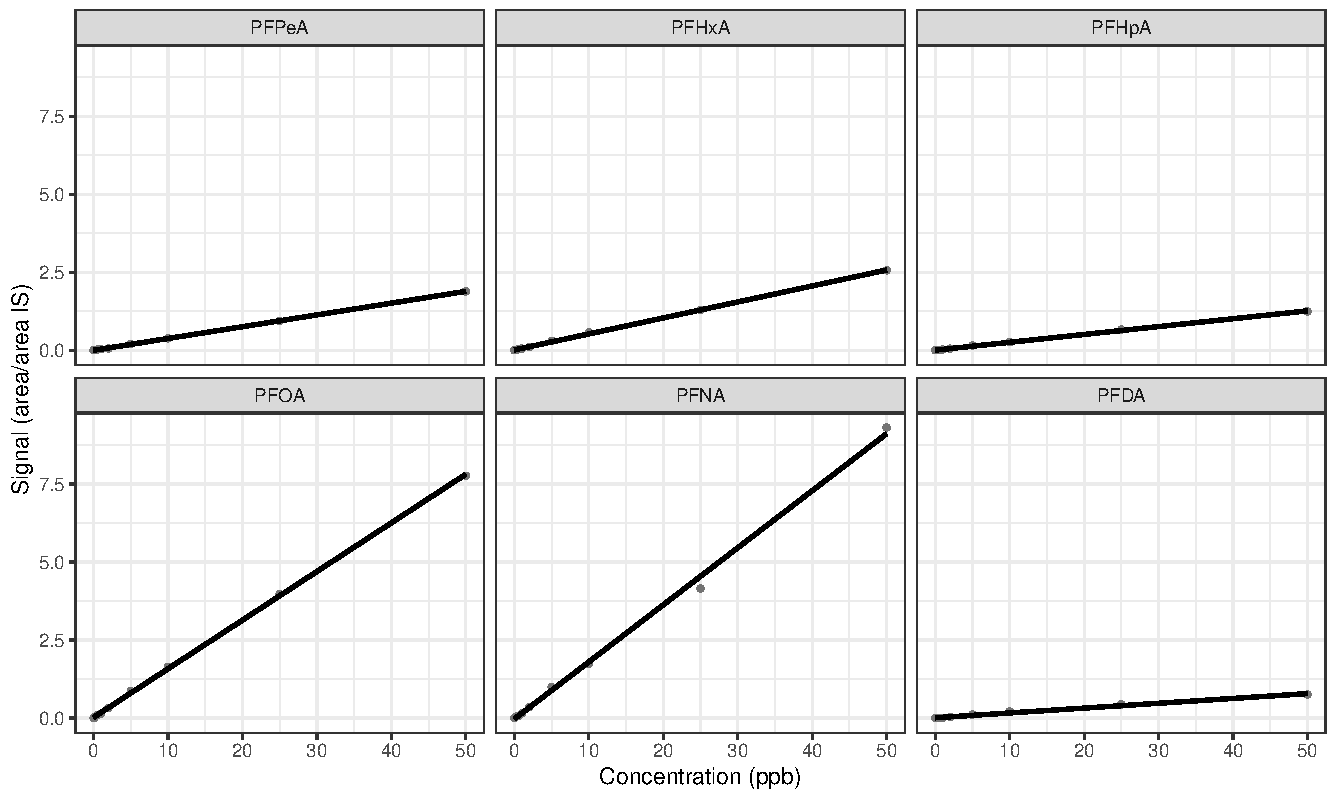
\includegraphics[width=0.7\textwidth]{R/figs/CC_all.pdf}
    \caption{Calibration curve solvent blank}
    \label{appfig:CC}
\end{figure}


\begin{figure}
    \centering
    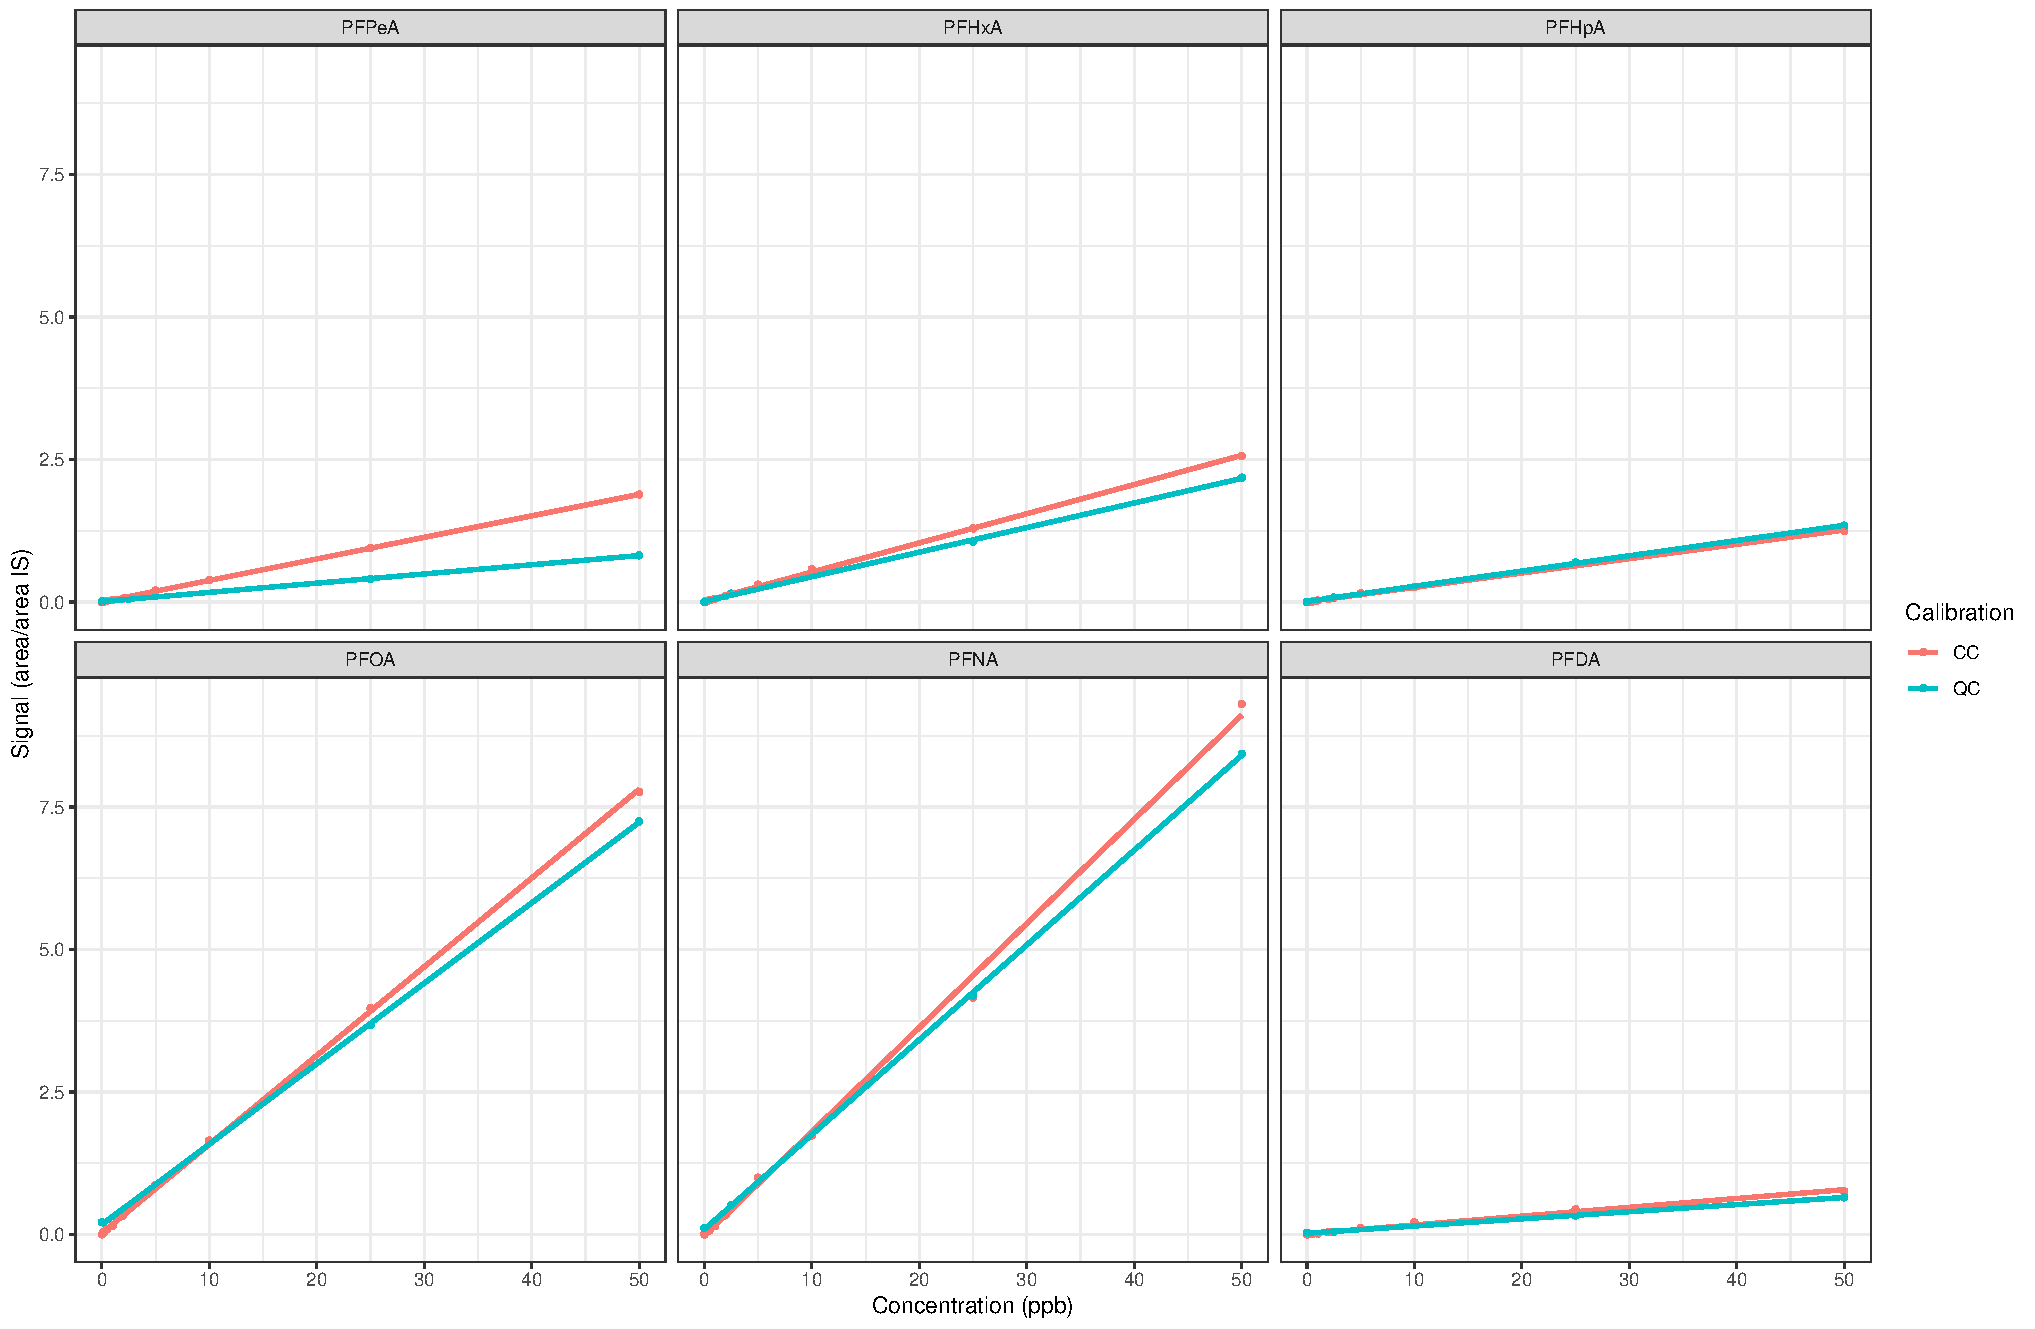
\includegraphics[width=0.7\textwidth]{R/figs/CCQC_matrixeffect.pdf}
    \caption{Matrix effect (ME) for the PFCAs where CC = calibration curve in solvent blank, QC = matrix matched calibration curve. QC in line with CC indicates no ME, QC \textgreater CC = ion enhancement, CC \textless QC = ion suppression.}
    \label{appfig:ME}
\end{figure}